\chapter{Perancangan}
\label{chap: Perancangan}

Pada bab ini akan dibahas mengenai perancangan perangkat lunak yang diimplementasi pada pohon kurikulum.

\section{Kebutuhan Masukan dan Keluaran}
\label{sec: Kebutuhan Masukan dan Keluaran}
Pada perancangan perangkat lunak pohon kurikulum dilakukan dengan membangkitkan dari JSON ke \textit{DOT}. Kebutuhan masukan dan keluaran perangkat lunak sebagai berikut:
\begin{itemize}
\item Masukan 
\begin{enumerate}
\item \textbf{data JSON}, berisikan JSON yang dipakai sebagai acuan dalam membangkitkan \textit{DOT}. data JSON dapat dilihat di lampiran B. Isi dari JSON adalah sebagai berikut :

\begin{enumerate}
\item \textbf{semester}, berisikan urutan semester 1 sampai semester 8. Setiap semester mempunyai isi sebagai berikut: 
\begin{itemize}
\item \textbf{kode}, berisikan kode mata kuliah.
\item \textbf{nama}, berisikan nama mata kuliah.
\item \textbf{sks}, memberitahukan kepada mahasiswa mata kuliah yang akan diambil memiliki beban berapa banyak.
\item \textbf{prasyarat}, isinya syarat tempuh atau lulus dari setiap mata kuliah.
\end{itemize}

\end{enumerate}

\item \textit{Engine DOT}, sebagai penerjemah dari JSON ke DOT.
\end{enumerate}

\item Keluaran\\
Keluaran dari perangkat lunak adalah grafik yang berbentuk pohon kurikulum dengan visualisasi menggunakan \textit{viz.js}. Pohon kurikulum akan menampilkan node semester 1 sampai semester 8. Kemudian di setiap semesternya terdapat node yang berisikan kode, sks, dan nama matakuliah. 
\end{itemize}

\section{Perancangan Perangkat Lunak Pohon Kurikulum}
\label{sec: Perancangan Perangkat Lunak Pohon Kurikulum}
Berikut rancangan pembuatan perangkat lunak pohon kurikulum:

\begin{enumerate}
\item Memanggil \textit{library}\\
Untuk membuat pohon kurikulum dibutuhkan \textit{library} sebagai bantuan untuk memanggil fungsi yang akan dijalankan. Dalam sebuah library umumnya memiliki perilaku spesifik. Perilaku spesifik ini diartikan sebagai sebuah spesifikasi masukan dan keluaran dari fungsi tersebut. Spesifikasi ini dapat mencakup tipe data (masukan maupun keluaran), paramter fungsi, dan banyak hal lain. Ada tiga \textit{library} yang digunakan pada pembuatan pohon kurikulum, yaitu \textit{viz.js, http, dan axios}. Fungsi dari masing - masing \textit{library} sebagai berikut:
\begin{itemize}
\item \textit{viz.js}, fungsinya sebagai visualisasi dalam bentuk grafik.
\item \textit{http}, fungsinya menjalankan \textit{server} di \textit{web} tanpa menggunakan program \textit{server web} seperti \textit{Apache}. 
\item \textit{axios}, \textit{library} untuk \textit{http request}, karena untuk mengakses data \textit{raw} di \textit{github} perlu \textit{request} data melalui \textit{http}.
\end{itemize} 
\item Memakai Node.js sebagai dasar untuk memanggil \textit{viz, http,} dan \textit{axios}.
\item Membuat rancangan pemanggilan DOT pada saat akan divisualisasikan. 
\item Membuat method untuk memanggil \textit{node} dan \textit{edge} yang akan digunakan pada saat pembuatan pohon kurikulum.
\end{enumerate}


\section{Perancangan Antarmuka Pohon Kurikulum}
\label{sec: Perancangan Antarmuka Pohon Kurikulum}
Untuk memenuhi kebutuhan interaksi antara pengguna dengan perangkat lunak, maka dirancanglah sebuah antarmuka berupa pohon kurikulum. Rancangan antarmuka dibuat dengan cara membangkitkan menggunakan \textit{viz.js}. Setelah itu pada saat pemanggilan antarmuka dapat diatur bentuk dan keluaran yang akan dipakai untuk membangkitkan pohon kurikulum. Beberapa opsi parameter yang dapat digunakan untuk merubah tampilan dari graf yang akan ditampilkan, yaitu dengan menggunakan \textit{engine} yang dapat dipakai pada \textit{Graphviz}, macam - macam \textit{engine} sebagai berikut: \textit{"circo", "dot", "fdp", "neato", "osage", atau "twopi"}. Selain \textit{engine} ada juga parameter pilihan. parameter ini mengatur apakah mata kuliah pilihan akan ditampilkan atau sebaliknya. Cara pemanggilan antarmuka sebagai berikut:

\begin{enumerate}
\item Cara \textit{default} pemanggilan \textit{url} sebagai berikut:
\begin{lstlisting}
localhost:8001/ 
\end{lstlisting}
Jika dilakukan pemanggilan seperti \textit{url} di atas maka keluarannya \textit{engine=dot} dan pilihan=false.

Contohnya dapat dilihat pada Gambar \ref{fig: wajib}
\begin{figure}[H]
		\centering
		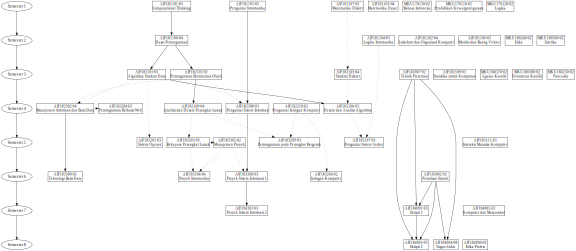
\includegraphics[scale = 0.5]{dot.png}
		\caption{DOT yang berisi Mata Kuliah Wajib saja}
		\label{fig: wajib}
\end{figure}	

\item Cara selanjutnya dengan menambahkan tanda tanya, \textit{url} sebagai berikut:
\begin{lstlisting}
localhost:8001/?engine=dot&pilihan=true
\end{lstlisting}

Jika dituliskan seperti \textit{url} di atas maka harus menentukan \textit{engine} dan pilihan. Hasilnya bisa sama atau berbeda dengan cara pemanggilan yang pertama. Pada pemanggilan \textit{url} di atas maka pohon kurikulum akan mengeluarkan graf yang memiliki \textit{engine = dot} dan pilihan=\textit{true}. Jika pilihan bernilai \textit{true} maka seluruh mata kuliah akan ditampilkan.

\end{enumerate}